% https://www.overleaf.com/learn/latex/Beamer#Using_a_colorthemev

% Inbuilt themes in beamer
\documentclass[8pt, aspectratio=169]{beamer}

\input{../template/macros/macros_general.tex}
\input{../template/macros/macros_math.tex}
\input{../template/symbols/symbols_NN.tex}
\input{../template/symbols/symbols_robot.tex}

% ~~~~~~~~~~~~~~~~~~~~~~~~~~~~~~~~~~~~~~~~~~~~~~~~~~~~~~~~~~~~~~~~~~~~~~~~~~~~~~
% Block options: block, alertblock, exampleblock
% ~~~~~~~~~~~~~~~~~~~~~~~~~~~~~~~~~~~~~~~~~~~~~~~


% % Theme choice:
% \usetheme{Antibes}
% % \usecolortheme{beaver}
%~~~~~~~~~~~~~~~~~~~~~~~~~~~~~~~~~~~~~~~~~~~~~~~~~~~~~~~~~~~~~~~~~~~~~~~~~~~~~~
% Use roboto Font (recommended)
% \usepackage[sfdefault]{roboto}
\usepackage[utf8]{inputenc}
\usepackage[T1]{fontenc}
%~~~~~~~~~~~~~~~~~~~~~~~~~~~~~~~~~~~~~~~~~~~~~~~~~~~~~~~~~~~~~~~~~~~~~~~~~~~~~~

%~~~~~~~~~~~~~~~~~~~~~~~~~~~~~~~~~~~~~~~~~~~~~~~~~~~~~~~~~~~~~~~~~~~~~~~~~~~~~~
% Define where theme files are located. ('/styles')
\usepackage{styles/fluxmacros}
\usefolder{styles}
% Use Flux theme v0.1 beta
% Available style: asphalt, blue, red, green, gray 
\usetheme[style=blue]{flux}
%~~~~~~~~~~~~~~~~~~~~~~~~~~~~~~~~~~~~~~~~~~~~~~~~~~~~~~~~~~~~~~~~~~~~~~~~~~~~~~

%~~~~~~~~~~~~~~~~~~~~~~~~~~~~~~~~~~~~~~~~~~~~~~~~~~~~~~~~~~~~~~~~~~~~~~~~~~~~~~
% Extra packages for the demo:
\usepackage{booktabs}
\usepackage{colortbl}
\usepackage{ragged2e}
\usepackage{schemabloc}
%~~~~~~~~~~~~~~~~~~~~~~~~~~~~~~~~~~~~~~~~~~~~~~~~~~~~~~~~~~~~~~~~~~~~~~~~~~~~~~
% \usepackage{calc}
% \usepackage{svg}
% \usepackage{media9}             %pdflatex, latex+dvips+ps2pdf, xelatex
% \usepackage{multimedia}
% \usepackage{animate}

% Title page details: 
\title{
    Imposing a Weight Norm Constraint for Neuro-Adaptive Control 
} 
\subtitle{
    \textit{IEEE European Control Conference (ECC) 2025}\\
}
\author{
  \textbf{Myeongseok Ryu}\inst{1}, Jiyun Kim\inst{2}, and Kyunghwan Choi\inst{1}
  }
\date{2025-06-25}
\institute{%
    \begin{minipage}[c]{\linewidth}
        \centering
        \inst{1}%
        Department of Mechanical and Robotics Engineering\\
        Gwangju Institute of Science and Technology
        \and
        \inst{2}%
        AI Graduate School\\
        Gwangju Institute of Science and Technology
  \end{minipage}
}
\titlegraphic{assets/MIC_Lab_logo_white.png}
% make institute font size smaller
\setbeamerfont{institute}{size=\normalsize}

\logo{
  \vspace{-.7cm}%
  
\includegraphics[height=0.3cm]{assets/kaist_logo.png}
  
\includegraphics[height=0.3cm]{assets/MIC_Lab_logo.png}
  \hspace{.6cm}%
  }

\AtBeginSection[]{%
  \frame<beamer>{ 
    \frametitle{Outline}   
    \tableofcontents[currentsection] 
  }
}

% \AtBeginSubsection[]{%
%   \begin{frame}
%   \vfill
%   \centering
%     \insertsectionhead
%     \\
%     \large\textbf{\insertsubsectionhead}
%   \vfill
%   \end{frame}
% }

\begin{document}

% Title page frame
% \begin{frame}
\titlepage 
% \end{frame}

% Outline frame
\begin{frame}{Outline}
    \tableofcontents
\end{frame}

% Lists frame
\section{Background and Contributions}

\subsection{Introduction to Neuro-Adaptive Control}

\begin{frame}{\insertsubsectionhead}{What is Neuro-Adaptive Control?}

  \textbf{Neuro-Adaptive Control}
  \small{
    \begin{itemize}
      \item \textbf{Neuro-adaptive control} (NAC) is a control strategy that combines \textbf{neural networks (NNs)} with \textbf{adaptive control} \cite{Farrell:2006aa}.
      \item Features of both \textbf{NNs} and \textbf{adaptive control} can be found in NAC.
    \end{itemize}
  }

  \begin{figure}
    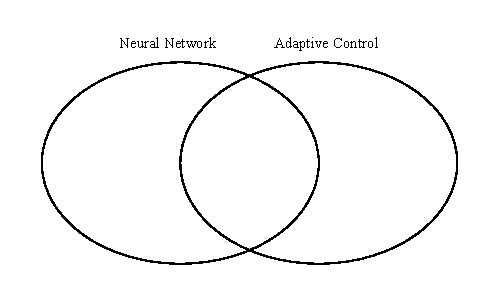
\includegraphics[width=0.65\textwidth]{figures/NAC.drawio.pdf}
  \end{figure}

\end{frame} 


\begin{frame}{\insertsubsectionhead}{What is Neuro-Adaptive Control?}

  \textbf{Advantages of Neuro-Adaptive Control}
  \small{
    \begin{itemize}
      \item \textbf{Adaptability}: NAC adapts to changing environments and system dynamics.
      \item \textbf{Stability Guarantee}: The closed-loop stability is ensured using \textit{Lyapunov stability theory}.
      \item \textbf{Online Learning Capability}: NAC adapts in \textit{real-time} to new data with stability guarantees.
      \item \textbf{Robustness}: NAC handles \textit{uncertainties and disturbances} effectively with adaptive control techniques.
    \end{itemize}
  }
  
\begin{figure}
  \label{fig:general_framework}
  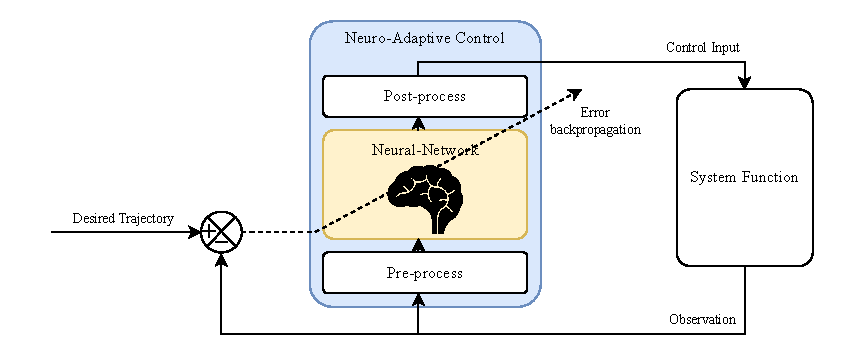
\includegraphics[width=0.65\textwidth]{figures/conv_nac.drawio.pdf}
  \caption{General framework of neuro-adaptive control (NAC).}
\end{figure}

\end{frame}

\begin{frame}{\insertsubsectionhead}{Existing Challenges in NAC}
  
  \textbf{Challenges}
  \small{
    \begin{itemize}
      \item \textbf{Optimality}: In general, the adaptation laws are driven with respect to the tracking error, which may not guarantee optimal performance.
      \item \textbf{Unpredictable Amplitude of Control input}: 
        \begin{itemize}
          \item The maximum amplitude of the NN weights is not predictable.
          \item This can result in unpredictable amplitude of the control input, which may lead to control saturation.
        \end{itemize}
      \item \textbf{Parameter Dependency}: 
      \begin{itemize}
        \item The performance of the NAC is highly dependent on the choice of parameters, such as learning rate and NN architecture.
      \end{itemize}
    \end{itemize}
  }

  \begin{figure}
    
\includegraphics[width=0.25\textwidth]{figures/KAIST-hi.png}
  \end{figure}

\end{frame}

\subsection{Literature Review}

\begin{frame}{\insertsubsectionhead}{Boundedness of NN Weights}
  
  In general, the NN outputs are bounded by limiting the maximum amplitude of the NN weights.

  \begin{enumerate}
    \begin{columns}[T,onlytextwidth]
        \column{0.49\textwidth}
          \item \textbf{Projection Operator}

          \begin{itemize}
            \item Cats 
            \item Dogs 
            \item Birds
          \end{itemize}

        \column{0.49\textwidth}
          \begin{figure}
            
\includegraphics[width=0.4\textwidth]{figures/KAIST-hi.png}
          \end{figure}
      \end{columns}

      \begin{columns}[T,onlytextwidth]
        \column{0.49\textwidth}
          \item \textbf{$\epsilon$-modification, and $\sigma$-modification}

          \begin{itemize}
            \item Cats 
            \item Dogs 
            \item Birds
          \end{itemize}

        \column{0.49\textwidth}
          \begin{figure}
            
\includegraphics[width=0.4\textwidth]{figures/KAIST-hi.png}
          \end{figure}
      \end{columns}
  \end{enumerate}
\end{frame}


\subsection{Literature Review}

\begin{frame}{\insertsubsectionhead}{Input Saturation}
  
  The input saturation is generally handled using an auxiliary system.

  \begin{enumerate}
    \begin{columns}[T,onlytextwidth]
        \column{0.49\textwidth}
          \item \textbf{Auxiliary Systems}

          \begin{itemize}
            \item Cats 
            \item Dogs 
            \item Birds
          \end{itemize}

        \column{0.49\textwidth}
          \begin{figure}
            
\includegraphics[width=0.4\textwidth]{figures/KAIST-hi.png}
          \end{figure}
      \end{columns}

      \begin{columns}[T,onlytextwidth]
        \column{0.49\textwidth}
          \item \textbf{Second?}

          \begin{itemize}
            \item Cats 
            \item Dogs 
            \item Birds
          \end{itemize}

        \column{0.49\textwidth}
          \begin{figure}
            
\includegraphics[width=0.4\textwidth]{figures/KAIST-hi.png}
          \end{figure}
      \end{columns}
  \end{enumerate}
\end{frame}


\subsection{Research Objectives}

\begin{frame}{\insertsubsectionhead}

  \textbf{Objective 1: Optimality}
  \begin{itemize}
    \item Formulate a constrained optimization problem to minimize the tracking error.
    \item Guarantee the stability of the system and the NN weights.
  \end{itemize}

  \textbf{Objective 2: Stability}
  \begin{itemize}
    \item Derive an adaptation law that guarantees the stability of the system.
    \item Ensure that the NN weights remain bounded during operation.
  \end{itemize}

  \textbf{Objective 3: Boundedness of }
  \begin{itemize}
    \item Ensure the controller is robust to uncertainties and disturbances.
    \item Validate the proposed method through numerical simulations.
  \end{itemize}

\end{frame}

\section{Proposed Method}

\subsection{Architecture of the Proposed Method}

\begin{frame}{\insertsubsectionhead}
  
  \begin{columns}
    
    \column{0.5\textwidth}
      
      \textbf{Target 2-link Robotic Manipulator System}:
      \begin{itemize}
        \item Control input saturation function $\mysat(\cdot)$.
        \item Desired trajectory $\mv{q}_d$ is given.
      \end{itemize}
        \begin{equation}
          \mm{M}\ddq + \mm{V}_m\dq + \mv{F} + \mv{G} + \mv{\tau}_d
          =
          \mysat(\mv{\tau})
        \end{equation}
      
      \textbf{Control Input}:
      \begin{itemize}
        \item NN's output $\mv{\Phi}$ is used as the control input.
        \item Consists of the estimated NN weights $\estwth$.
      \end{itemize}
      \begin{equation}
        \mv{\tau} := \mv{\Phi}(\mv{q}_n; \estwth)
      \end{equation}

      \textbf{Deep Neural Network (DNN)}:
      \begin{itemize}
        \item $k$ layers with $\estwth_i:=\myvec(\estwV_i)$.
        \item Activation function: $\phi(\cdot):=tanh(\cdot)$.
        \begin{equation}
          \mv{\Phi}(\mv{q}_n; \estwth)
          :=
          \begin{cases}
              \estwV_i^\top \act_i(\estNN_{i-1}), 
              &
              i\in\{1,\dots ,k\},
              \\
              \estwV_0^\top {\q}_n,
              &
              i=0
              ,
          \end{cases}
        \end{equation}
      \end{itemize}

    \column{0.5\textwidth}  

      \begin{figure}
        \includegraphics[width=0.8\textwidth]{figures/Controller.drawio.pdf}
        \caption{Architecture of the proposed method.}
      \end{figure}

      \begin{figure}
        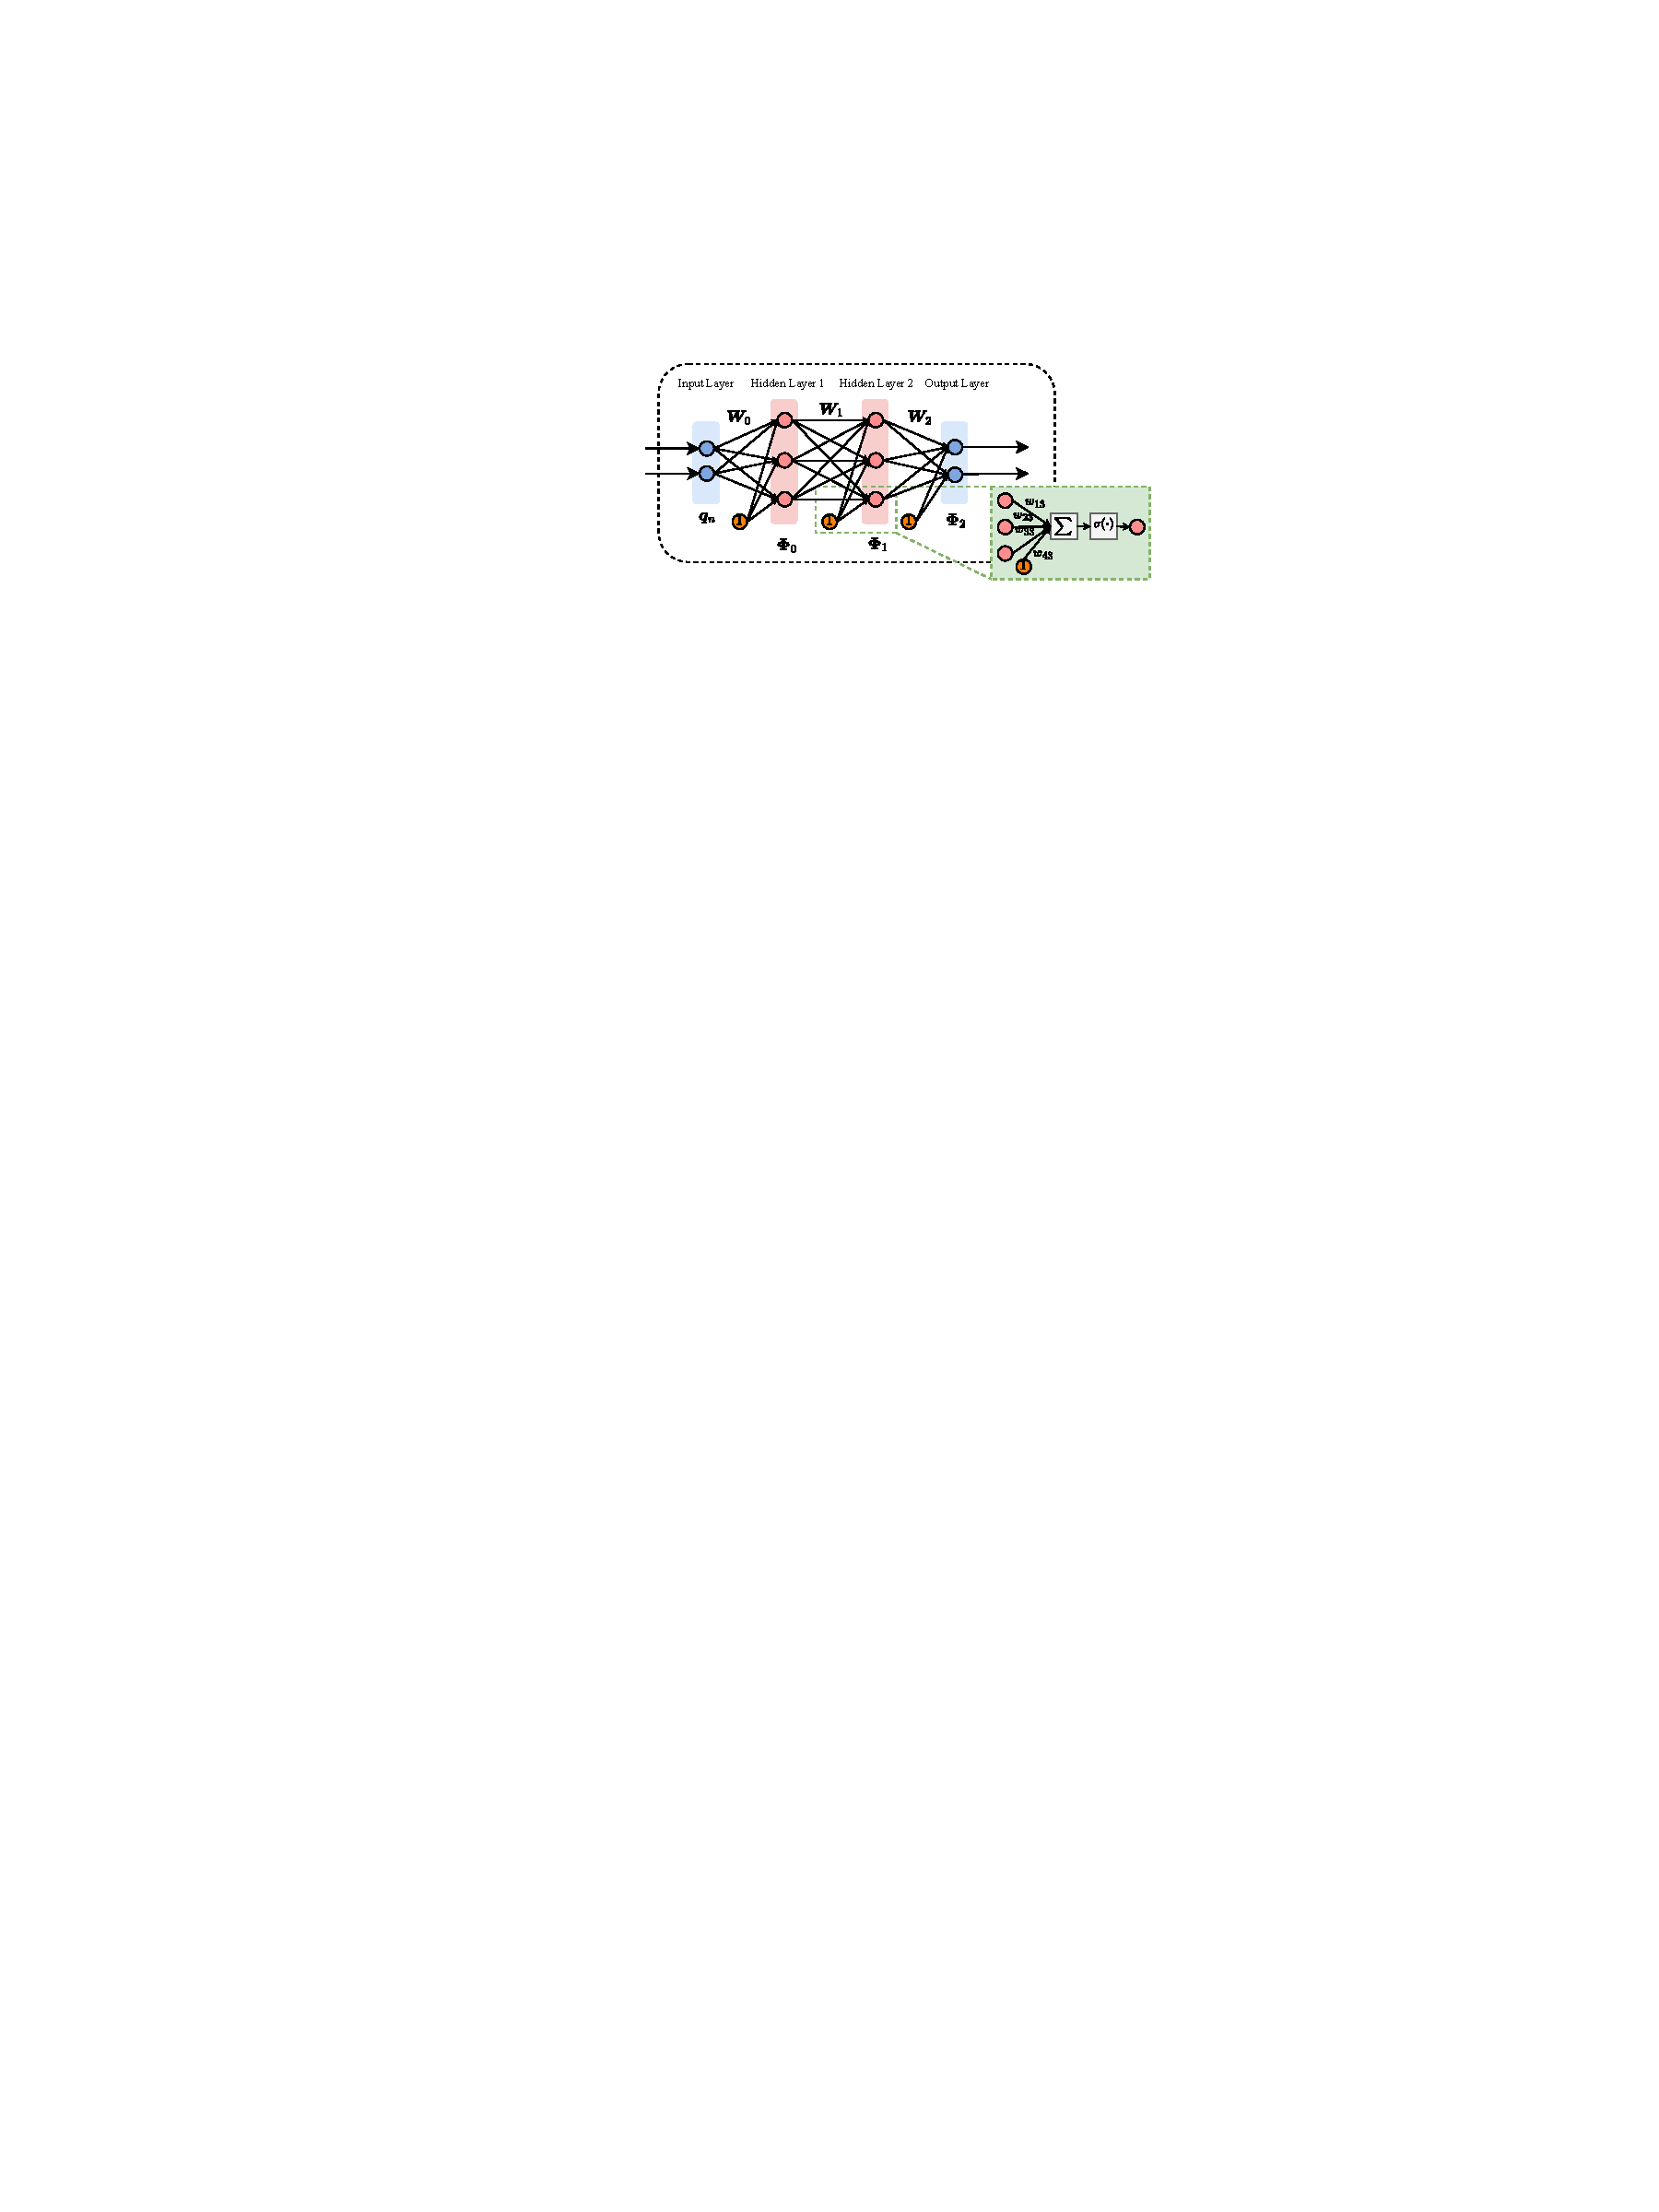
\includegraphics[width=0.7\textwidth]{figures/DNN.drawio.pdf}
        \caption{Architecture of the DNN.}
      \end{figure}

  \end{columns}

    \let\thefootnote\relax\footnote{
      \textit{Notations}: 
        $\mv{q}\in\R^n$: Joint position, $\mm{M}$: Inertia matrix, $\mm{C}$: Coriolis matrix, $\mm{G}$: Gravity vector, $\mv{\tau}$: Control input, $\estwth$: Estimated NN weights.
        $\estwth$: Estimated NN weights, $\mv{e}$: Tracking error, $\mv{\tau}_d$: Disturbance, $\mysat(\cdot)$: Saturation function.
      }

\end{frame}

\subsection{Problem Formulation}

\begin{frame}{\insertsubsectionhead}{Optimization Problem}

\begin{columns}

  \column{0.45\textwidth}

    \textbf{Optimization Problem Statement}:

    \begin{itemize}
      \item \textbf{Find} NN weights $\estwth$,
      \item That \textbf{minimize} objective function $J(\cdot)$,
        \begin{equation}
          J(\mv{r}) := \frac{1}{2} \mv{r}^\top \mv{r}.
        \end{equation}
        \begin{itemize}
          \item where $\mv{r} := \ddt\mv{e} + \Lambda\mv{e}$ is the filtered tracking error,
        \end{itemize}
      \item while satisfying the following \textbf{constraints}:
        \begin{itemize}
          \item Boundedness of the NN weights $\estwth$.
          \item Saturation of the control input $\mv{\tau}$.
        \end{itemize}
    \end{itemize}

  
  \column{0.5\textwidth}

    \begin{block}{Considered Constraints}

      \begin{itemize}
        \item \textbf{Weight Boundedness}: 
          \begin{equation}
            c_{\theta_i}
            :=
            \norm{\estwth_i}^2 - \bar{\theta_i}^2 \le 0
            , 
            \forall i\in\{0,\ldots,k\}
          \end{equation}

        \item \textbf{Control Input Saturation}: 
          \begin{itemize}
            \item Input bound constraint:
            \begin{equation}
              c_{\overline{\tau}_i}
              :=
              \tau_i - \overline{\tau_i}
              \le 
              0
              ,
              c_{\underline{\tau}_i}
              :=
              \underline{\tau_i} - \tau_i
              \le 
              0
            \end{equation}
            \item Input norm constraint:
            \begin{equation}
              c_{\mv{\tau}}
              :=
              \norm{\mv{\tau}}^2 - \overline{\tau}^2
              \le
              0
            \end{equation}
        \end{itemize}
      \end{itemize}
      
    \end{block}

  \end{columns}

  \let\thefootnote\relax\footnote{
    \textit{Notations}: 
    $\Lambda\in\R_{>0}^{n\times n}$: filtering matrix
  }

\end{frame}

\begin{frame}{\insertsubsectionhead}{Optimization Problem}

  \begin{columns}

    \column{0.5\textwidth}
      
      \centering
      \begin{minipage}{0.9\textwidth}%
        \begin{block}{Optimization Problem}%


          \begin{equation}
            \begin{matrix}
              \min_{\estwth} J(\mv{r};\estwth)
              \\\ \\
              \text{s.t. } c_{j}(\estwth) 
              \le 
              0
              ,
              \forall j\in\mathcal{J}
            \end{matrix}
          \end{equation}

        \end{block}
      \end{minipage}

    \column{0.5\textwidth}

      \centering
      \begin{minipage}{0.9\textwidth}%
        \begin{block}{MinMax Problem}%
          

          \begin{equation}
            \begin{matrix}
              \min_{\estwth}\max_{[\lambda_j]_{j\in\mathcal{J}}} L(\cdot)
              \\\ \\
              \text{where }
              L(\mv{r},\estwth,[\lambda_j]_{j\in\mathcal{J}})
              :=
              J(\mv{r};\estwth)
              +
              \sum_{j\in\mathcal{J}} \lambda_j c_j(\estwth)
            \end{matrix}
          \end{equation}

        \end{block}
      \end{minipage}

  \end{columns}

\end{frame}

\subsection{Adaptation Law Derivation}

\begin{frame}{\insertsubsectionhead}{Steepest Descent/Ascent Method}

  \begin{columns}

    \column{0.5\textwidth}
      
      \begin{minipage}{0.9\textwidth}%
        For the min/max problem, the steepest descent/ascent method is used to derive the adaptation law.
      \end{minipage}

      \vspace{0.5cm}

      \begin{minipage}{0.9\textwidth}%
        \textbf{Steepest Descent Method for $\estwth$}:
        \begin{equation}
          \ddtt\estwth
          =
          -\alpha 
          \pptfrac{L}{\estwth}
        \end{equation}

        \textbf{Steepest Ascent Method for $\lambda_j$}:
        \begin{equation}
          \ddtt\lambda_j = 
        \end{equation}
      \end{minipage}

    \column{0.5\textwidth}

      \centering
        \begin{block}{Adaptation Law}%

        \begin{subequations}
            \begin{align}
                    \ddt {{\estwth}}
                    &
                    =
                    -\alpha 
                    \ppfrac{L}{{\estwth}}
                    =-\alpha 
                    \left(
                        \ppfrac{J}{{\estwth}}
                        +
                        \sum_{j\in\mathcal{I}}
                        \lambda_j 
                        \ppfrac{c_j}{\estwth}
                    \right),
                    \\
                    \ddt\lambda_j
                    & 
                    = 
                    \beta_j
                    \ppfrac{L}{\lambda_j} 
                    = 
                    \beta_j c_j ,
                    \quad\quad\quad\quad      \      
                    \forall j\in\mathcal I,
                    \\
                    \lambda_j 
                    & 
                    = 
                    \max(\lambda_j,0) ,
            \end{align}
        \end{subequations}

        \end{block}

  \end{columns}

\end{frame}

\subsection{Stability Analysis}

\begin{frame}{\insertsubsectionhead}{Lyapunov Stability Analysis}

  \begin{block}{Theorem 1}
    For the dynamical system described in (1), the neuro-adaptive controller in (2) with the weight adaptation laws in (12) ensure the boundedness of the filtered error $\mv{r}$ and the weight estimate $\estwth$, under the control input constraints satisfying Assumption 1 and 2. This holds under the weight norm constraint (5).
  \end{block}

  \begin{exampleblock}{Assumption 1}
    The constraint functions $c_j(\estwth),\forall j\in\mathcal{I}$, are convex in the $\tau$-space and satisfy $c_j(\estwth)\le0$ and $c_j(\idealwth)\le0$.
  \end{exampleblock}

  \begin{exampleblock}{Assumption 2}
    The selected constraints satisfy the Linear Independence Constraint Qualification (LICQ) \cite[Chap. 12 Def. 12.1]{Nocedal:2006aa}.
  \end{exampleblock}

  Proof of Theorem 1 is omitted due to space limitations. The detailed proof can be found in \cite{}.

\end{frame}

\section{Numerical Validation}

\subsection{Simulation Setup}
\begin{frame}{\insertsubsectionhead}{2-Link Robotic Manipulator}
    
  \begin{figure}
    \centering
    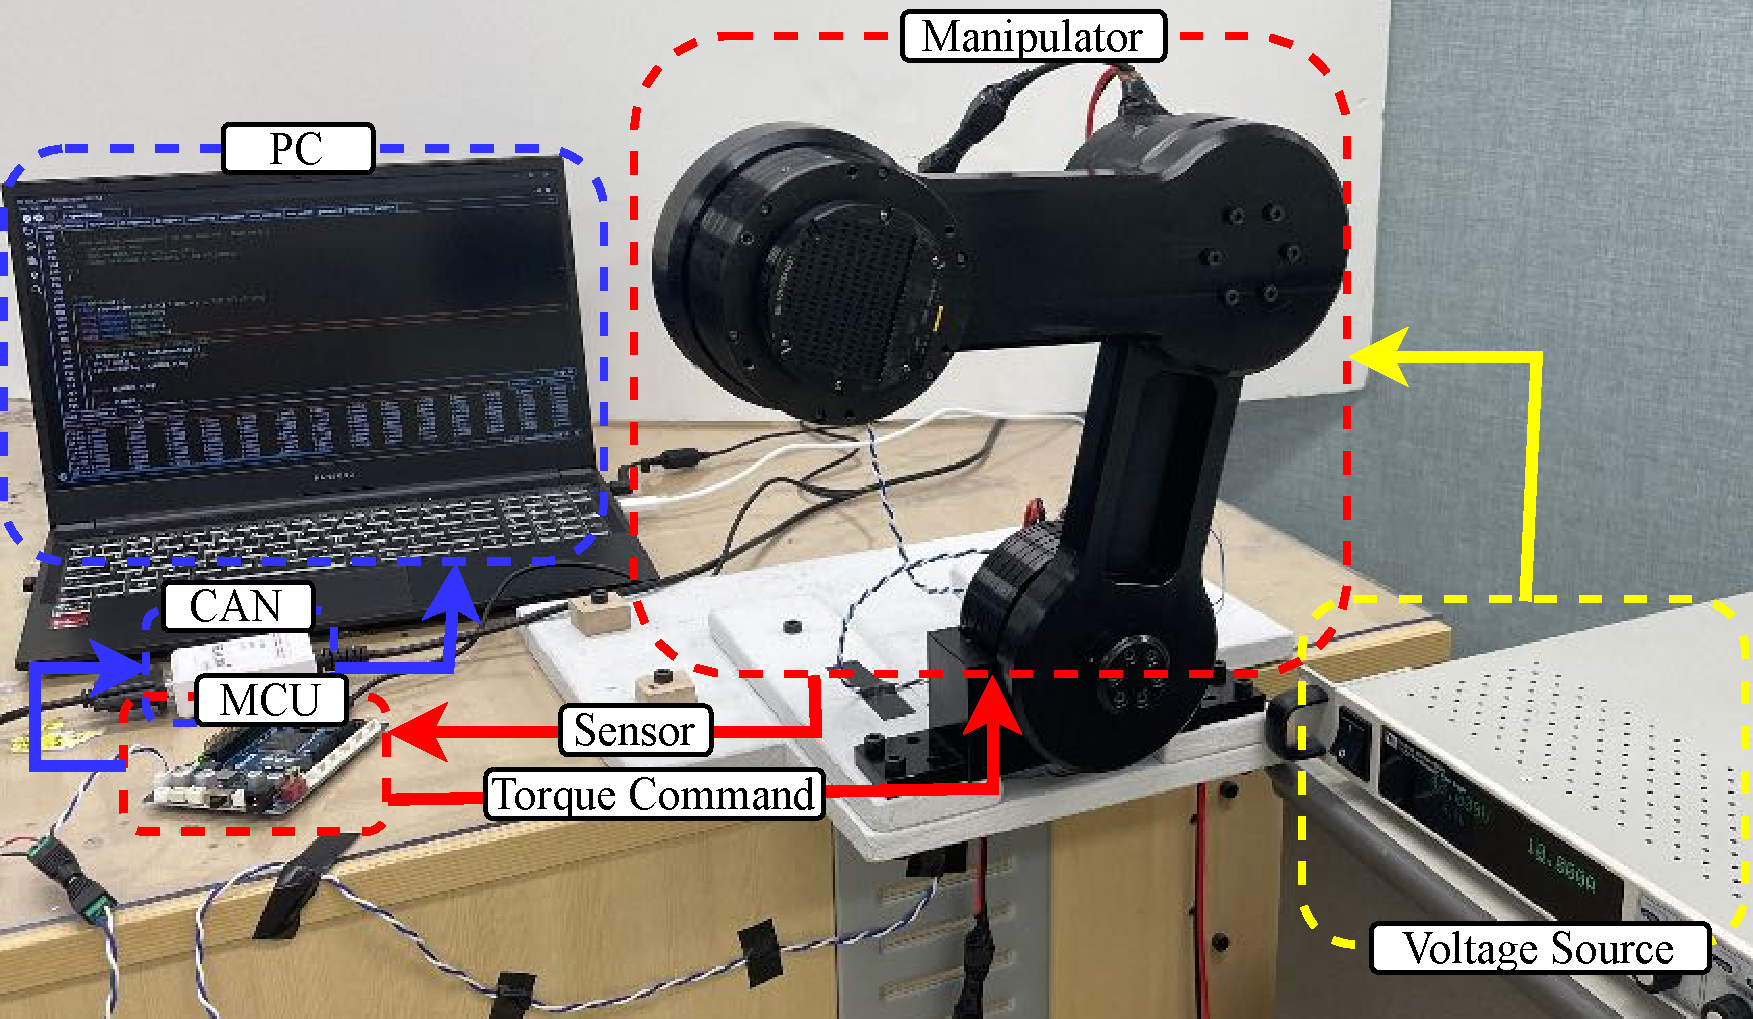
\includegraphics[width=0.5\textwidth]{figures/exp_set.drawio.png}
    \caption{2-Link Robotic Manipulator}
  \end{figure}

  \let\thefootnote\relax\footnote{
    \textit{Notations}: 
      $\mv{q}$: Joint position, $\mv{\dot{q}}$: Joint velocity, $\mv{\tau}$: Control input, $\mm{M}$: Inertia matrix, $\mm{C}$: Coriolis matrix, $\mm{G}$: Gravity vector.
  }


\end{frame}

\subsection{Simulation Results}

\begin{frame}{Representative Simulation Results}

  % % \movie[width=3cm,height=2cm,poster]{}{overall.mp4}
  % \begin{figure}
  %   \centering
  %   \href{https://youtu.be/U5uDbJQkGY8}{
  %     
\includegraphics[width=.1\textwidth]{figures/KAIST-hi.png}
  %   }
  % \end{figure}

  % \animategraphics[loop,width=4cm]{gifs/overall-}
  % \animategraphics[loop,width=4cm]{10}{gifs/overall-}{0}{10}


\end{frame}

\begin{frame}{Box-and-Whisker Plots}
  
  \begin{columns}
    \column{0.5\textwidth}
      \begin{figure}
        \includegraphics[width=\textwidth]{figures/BoxWhisker.drawio.png}
        \caption{Parameter dependencies of the proposed method.}
      \end{figure}

    \column{0.5\textwidth}
      \begin{table}
        \caption{Largest cities in the world (source: Wikipedia)}
        \begin{tabular}{@{} lr @{}}
          \toprule
          City & Population\\
          \midrule
          Mexico City & 20,116,842\\
          Shanghai & 19,210,000\\
          Peking & 15,796,450\\
          Istanbul & 14,160,467\\
          \bottomrule
        \end{tabular}
    \end{table}
    
  \end{columns}

\end{frame}

\begin{frame}{Parameter Dependencies}

  \begin{columns}

    \column{0.33\textwidth}
      \begin{figure}      
        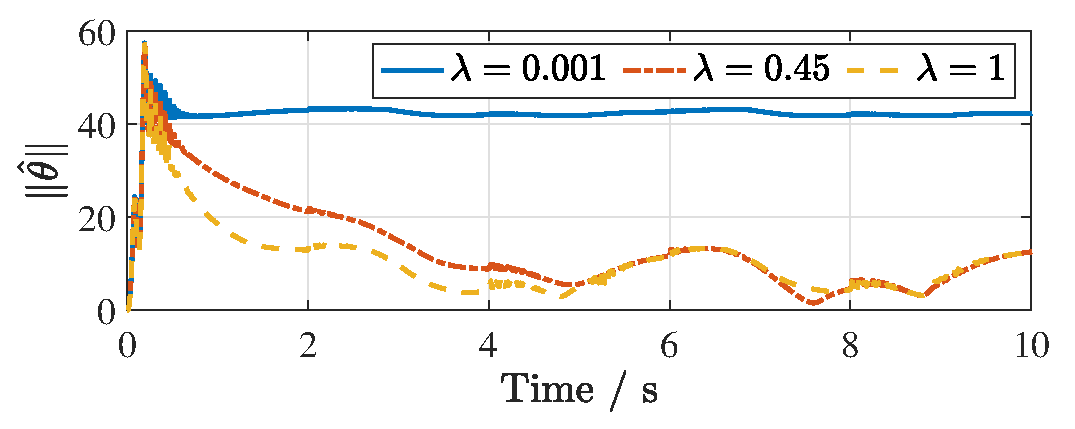
\includegraphics[width=0.99\textwidth]{figures/ECC/fig9.eps}
        \caption{Weight norms of NAC-L2}
      \end{figure}
      
    \column{0.33\textwidth}

      \begin{figure}
        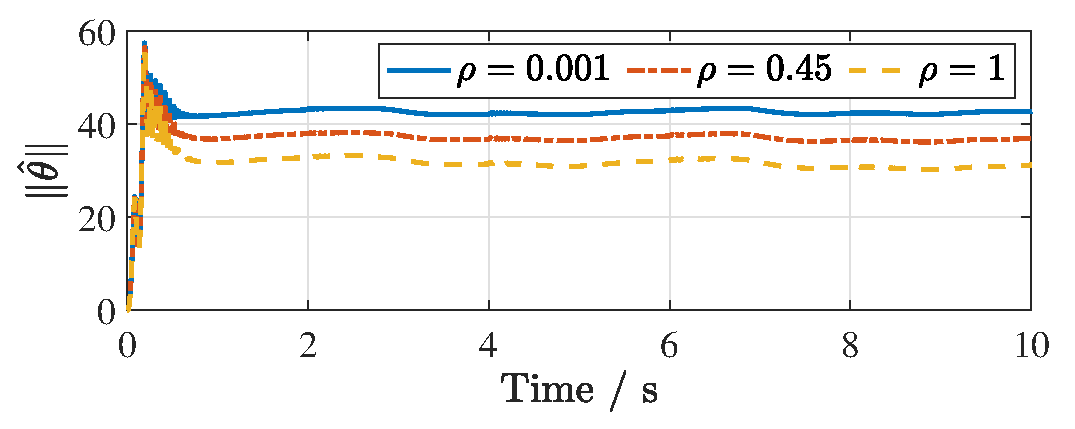
\includegraphics[width=0.99\textwidth]{figures/ECC/fig10.eps}
        \caption{Weight norms of NAC-eMod}
      \end{figure}

    \column{0.33\textwidth}

      \begin{figure}
        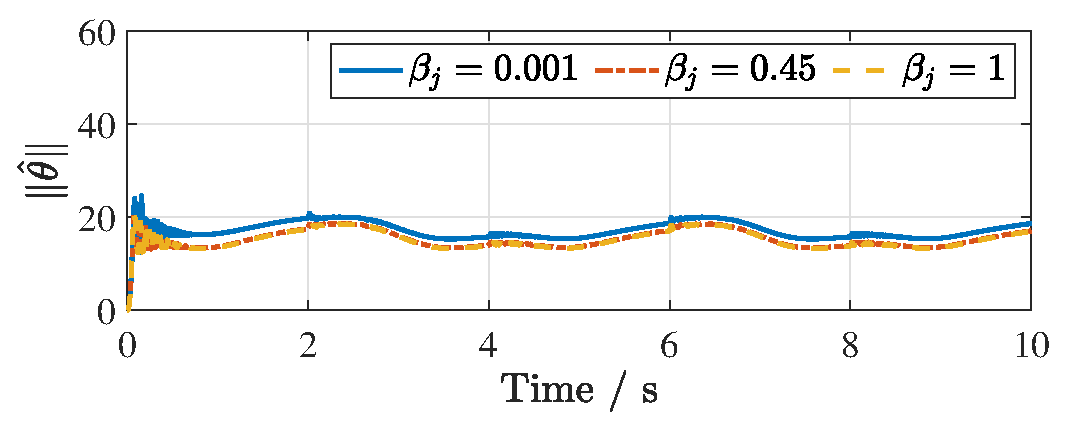
\includegraphics[width=0.99\textwidth]{figures/ECC/fig8.eps}
        \caption{Weight norms of NAC-CO}
      \end{figure}
    
  \end{columns}

  The weight norms of the proposed method (NAC-CO) are bounded, while ...

\end{frame}

\begin{frame}{Parameter Dependencies}

  \begin{columns}

    \column{0.33\textwidth}
      \begin{figure}      
        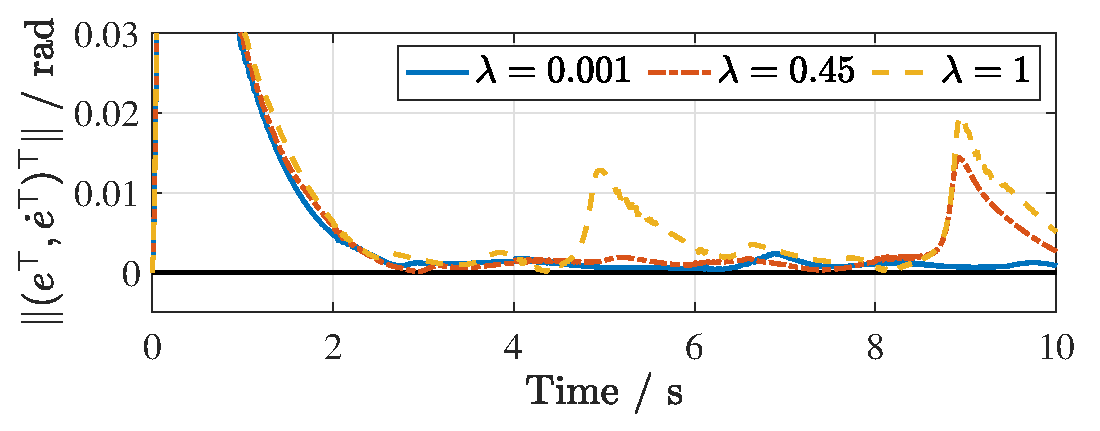
\includegraphics[width=0.99\textwidth]{figures/ECC/fig6.eps}
        \caption{Tracking error of NAC-L2}
      \end{figure}
      
    \column{0.33\textwidth}

      \begin{figure}
        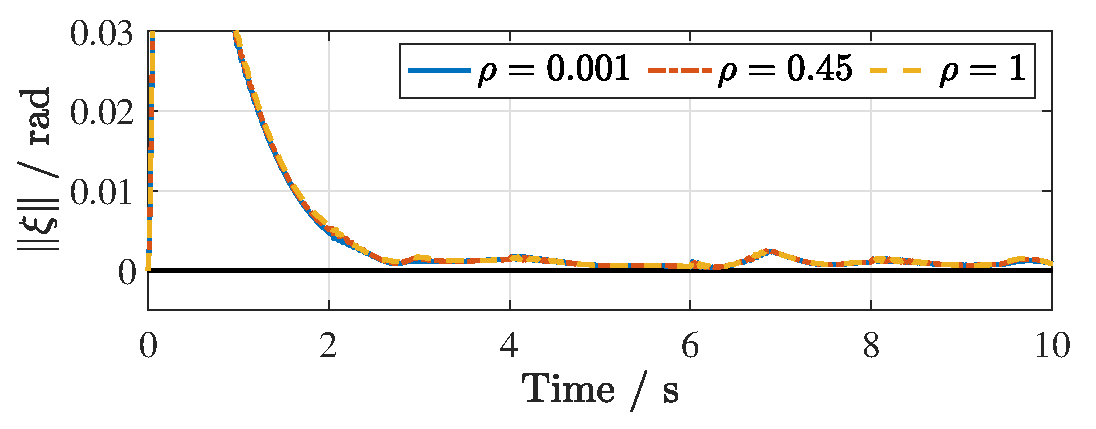
\includegraphics[width=0.99\textwidth]{figures/ECC/fig7.eps}
        \caption{Tracking error of NAC-eMod}
      \end{figure}

    \column{0.33\textwidth}

      \begin{figure}
        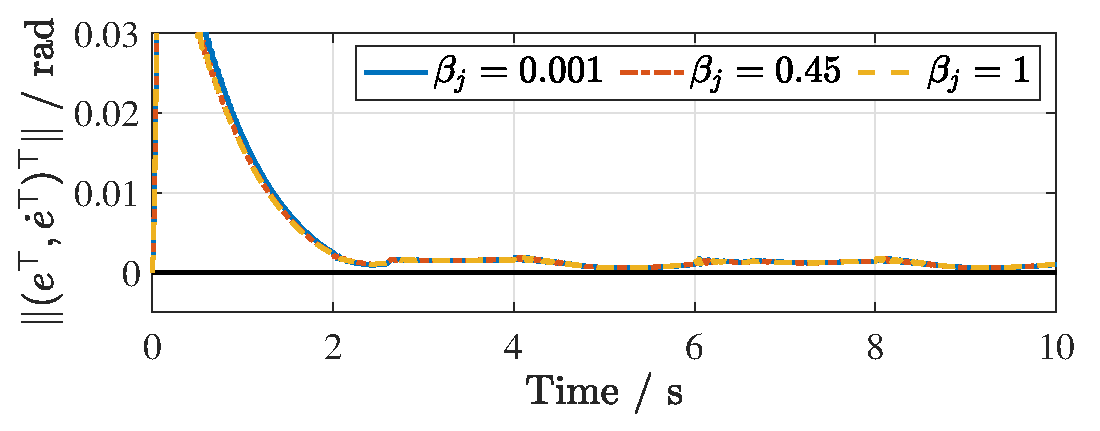
\includegraphics[width=0.99\textwidth]{figures/ECC/fig5.eps}
        \caption{Tracking error of NAC-CO}
      \end{figure}
    
  \end{columns}

  The Tracking error ...

\end{frame}

\section{Conclusion}

\subsection{Conclusion and Future Work}

\begin{frame}{Conclusion}
    
  \textbf{Summary of Contributions}
  \begin{itemize}
    \item Proposed a novel constrained optimization-based neuro-adaptive control (CONAC) method.
    \item Adaptation laws are derived using constrained optimization method.
    \item The proposed method guarantees the stability of the system and the boundedness of the NN weights.
    \item Feasibility of the proposed method is validated through numerical simulations and real-time experiments.
  \end{itemize}

  \textbf{Future Work}
  \begin{itemize}
    \item Extend the proposed method to state constraints.
    \item Enhance the robustness and flexibility of the proposed method for various systems.
  \end{itemize}

\end{frame}

\section{}
\begin{frame}{}
    \centering \Large
    \emph{Thank you for your attention!}
\end{frame}

\begin{frame}[allowframebreaks]{References}

  \bibliography{../template/refs}
  \bibliographystyle{ieeetr}

\end{frame}

\end{document}